\section{Terrain Generation}

The very first option in the application is to generate the terrain.
The terrain is generated by creating a mesh with height values gathered from a random noise map.
Before and after the terrain is generated can be seen in picture \ref{fig:no_terr} and \ref{fig:terr}.

Certain attributes of the terrain can be adjusted by the user, those options being:

\begin{easylist}
 @ Sea level: increases or decreases the water level
 @ Offset X and Z: slides along the respective axis in the noise map, changing the height values of the terrain.
 @ Size X and Z: Adjusts the size of the entire terrain.
\end{easylist}

\begin{figure}[H]
  \centering

  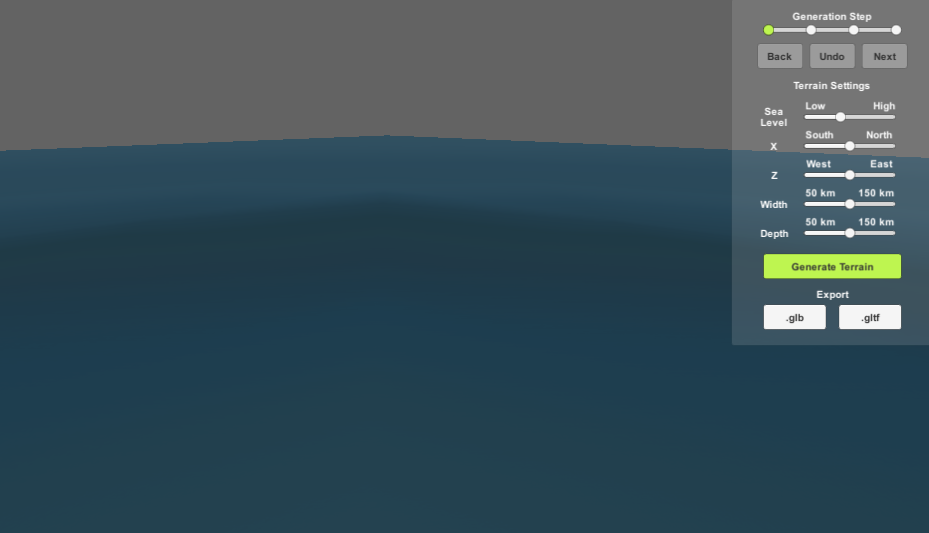
\includegraphics[width=0.7\textwidth]{figure/terrain_not_generated.png}
  \caption{The state before Generate Terrain button has been pressed. The water is visible from the very beginning.}

  \label{fig:no_terr}
\end{figure}

\begin{figure}[H]
  \centering

  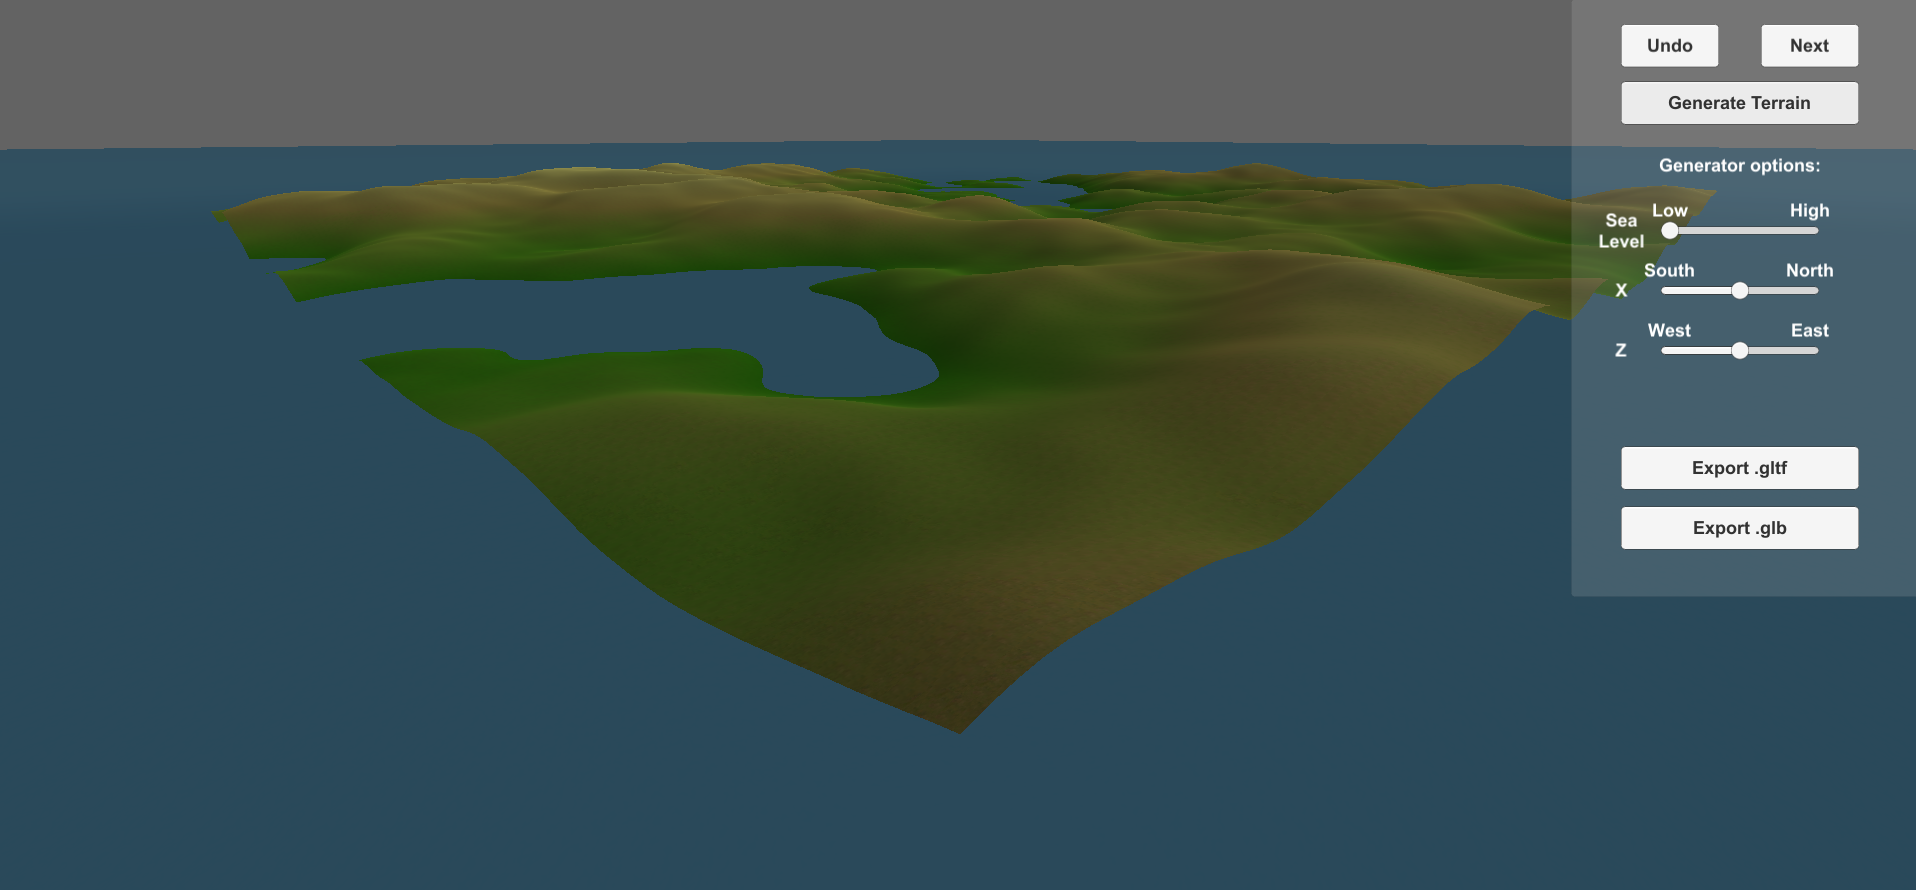
\includegraphics[width=0.7\textwidth]{figure/terrain_generated.png}
  \caption{The state after Generate Terrain button has been pressed.}

  \label{fig:terr}
\end{figure}

 
The water is a large plane which clips through the terrain, which worked well as a simple way to mimic real world water level.

The terrain contains one singular texture, which is repeated several times with random rotation.
This solution is not perfect, but it was the most effortless way to avoid creating a custom shader while also making the terrain look decent.
